\chapter{Planificación}

\section{Metodología utilizada}
Para el desarrollo del proyecto he elegido la \textbf{metodología SCRUM}.
Esta metodología es una de las más utilizadas en la actualidad y consiste en unas prácticas que permiten un trabajo de entregas que se va incrementando para el desarrollo de un producto. \\
La gran característica de esta metodología y por lo que recibe el nombre es su agilidad ya que consiste en presentar una serie de objetivos y/o requisitos necesarios, se les asigna una prioridad y se asigna al personal que va a trabajar en el proyecto.
Además otra característica es que el cliente va a poder empezar a utilizar el producto porque se va a ir desarrollando por partes por así decirlo.

Después se hace una planificación en la que se hace una estimación de los tiempos de entrega.
A partir de ahí estos requisitos que bien pueden ser historias de usuario, tareas de mantenimiento o correción de bugs del proyecto se van realizando.
 
\section{Seguimiento del desarrollo}

Para el seguimiento y gestión del desarrollo he utilizado el software de control de versiones
git en la plataforma Github. Esta plataforma me permite mediante un kanban organizar todo el proyecto
y tener un listado de requerimientos mediante historias de usuarios y tareas pendientes (issues) asignandoles
prioridad, asignandoselas a usuarios aunque en este caso todas estarán asignadas a mi ya que es un proyecto personal 
y más posibilidades.

Además para estar en contacto con mi tutor, he utilizado un Bot de Telegram que he conectado con mi repositorio y 
configurado para que cada commit o creación/cierre de issues se notifique en un grupo de telegram en el que estamos mi tutor y yo
junto con dicho Bot.

\subsection{Kanban}

Se ha creado un proyecto de GitHub y se ha utilizado una tabla Kanban para gestionar las historias de usuario y las issues del proyecto.

El Kanban del proyecto puede verse en el siguiente enlace:
\url{https://github.com/josemip98/TFG/projects/1}

\begin{figure}[H]
  	\centering
  	\noindent\makebox[\textwidth]{
	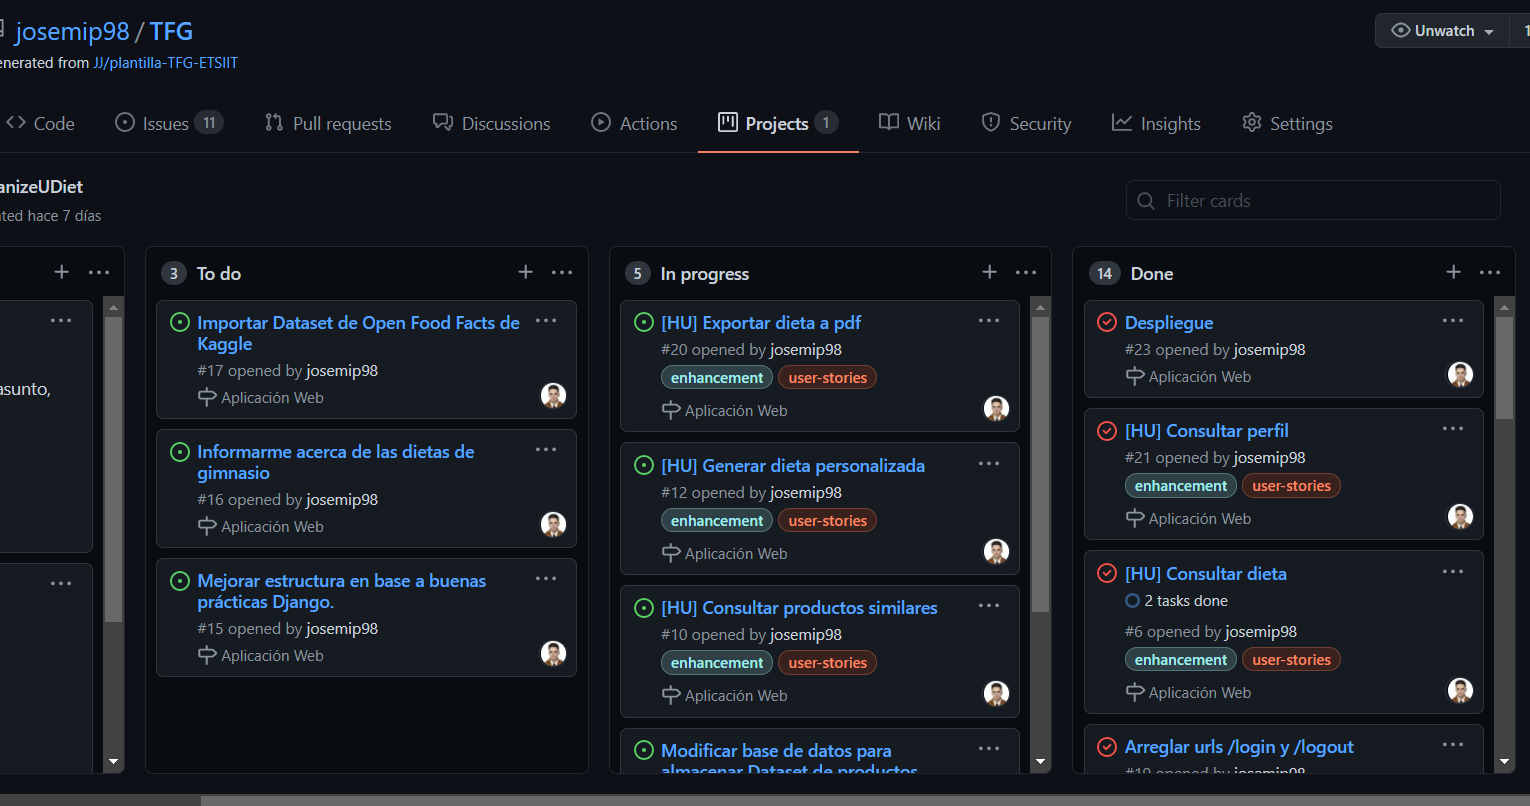
\includegraphics[scale=0.4]{kanban.png}}
  	\caption{Tabla Kanban del proyecto.}
	\end{figure}

\subsection{Historia de usuario}
Una historia de usuario es \textbf{una funcionalidad que el usuario espera}.
El modelo a seguir para la creación de historias de usuario es:

\textit{Como usuario/desarrollador quiero poder [funcionalidad] para [razón dicha funcionalidad].}

Además podemos añadir tareas que necesitamos cumplir para completar la historia de usuario o detalles técnicos.

\begin{figure}[H]
	\centering
	\noindent\makebox[\textwidth]{
	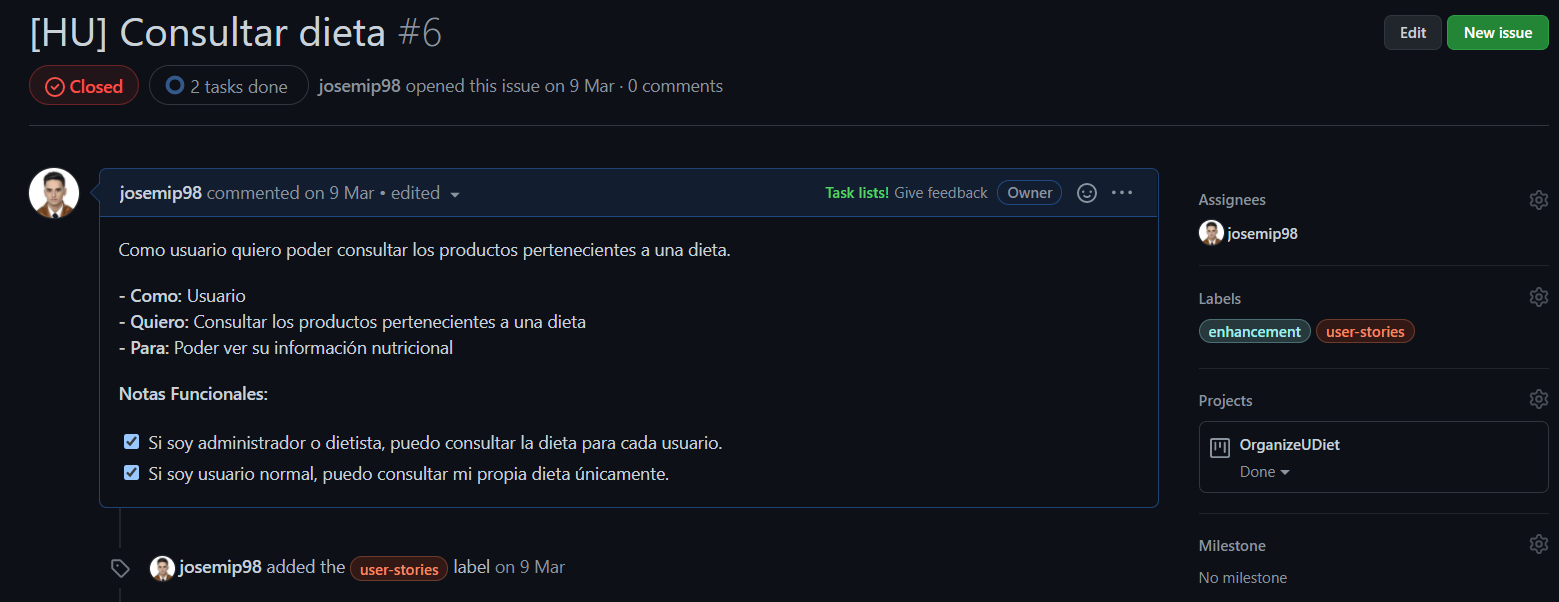
\includegraphics[scale=0.4]{hu.png}}
	\caption{Ejemplo historia de usuario.}
  	\end{figure}

\subsection{Issues}
Las issues pueden ser correción de bugs, tareas que sean necesarias para el desarrollo o mantenimiento del proyecto.

\begin{figure}[H]
	\centering
	\noindent\makebox[\textwidth]{
	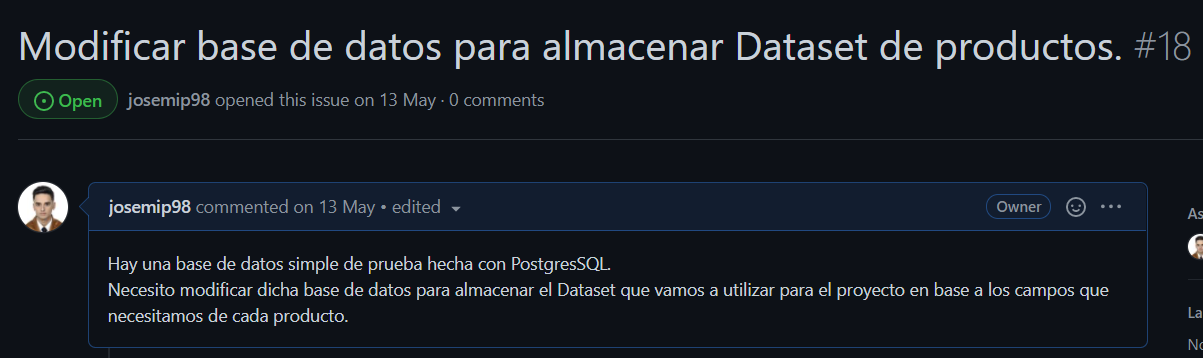
\includegraphics[scale=0.4]{issue.png}}
	\caption{Ejemplo de issue.}
  	\end{figure}

\subsection{Etiquetas}

Las etiquetas son la forma de categorizar las issues pendientes ya sea asignandoles prioridad o describiendo si es una issue de documentación, si es un bug, historia de usuario...
Además podemos crear etiquetas a nuestro gusto según las necesidades que tengamos.

\begin{figure}[H]
	\centering
	\noindent\makebox[\textwidth]{
	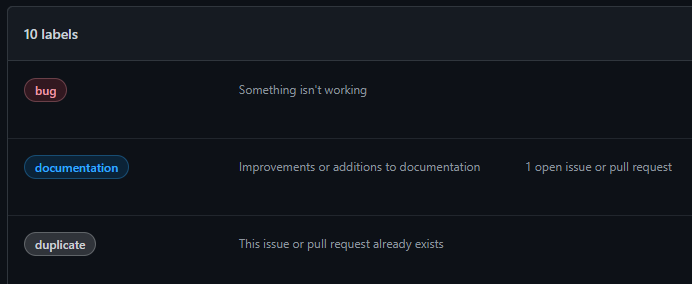
\includegraphics[scale=0.4]{etiquetas.png}}
	\caption{Ejemplo de etiquetas.}
	\end{figure}